\section{What information do rodents extract from sound?}
\label{sec:features}

To say that a sound is biologically significant is to say something about a receiver: what it extracts from the sound, and how that information shapes what it does next. It is not a statement about whether the sound is ``natural'' or ``alarming.'' Studies of rodent receivers keep returning to the same acoustic dimensions: carrier frequency and bandwidth, sound level, frequency and amplitude modulation, the temporal envelope, syllable and bout structure, call rate, harsh or noisy (nonlinear) components, and cues to the caller's identity. A natural call bundles all of these. Comparing a natural call with an artificial one therefore rarely shows which property mattered. And when a simplified sound reproduces a response, it remains open whether simplification stripped away meaning or simply isolated the features that were sufficient for that response.

\subsection{Acoustic salience is not ecological meaning}
\label{sec:features-salience}

Natural calls often beat poorly matched controls but fail to beat controls matched on the features the receiver actually uses. In food-restricted rats, natural 50-kHz calls evoked approach and a transient rise in nucleus accumbens dopamine, whereas natural 22-kHz calls and noise matched in duration and amplitude evoked neither \citep{WilluhnEtAl2014}. That shows the rats distinguished calls from that noise; it does not show which acoustic property was necessary. Pure-tone approximations of 50-kHz calls, lacking natural frequency and amplitude modulation, still draw rats toward the speaker, especially adults \citep{WohrSchwarting2007}. Natural 22-kHz and 50-kHz calls generally produce larger vocal, cardiac, and locomotor effects than computer-generated tones, but in the same direction, and housing condition changes the size of the effect \citep{OlszynskiEtAl2020}. In the amygdala, frequency-matched tones reproduce most of the neural discrimination between the two call types in naïve rats \citep{ParsanaEtAl2012a}. The inference these results support is narrower than ``natural calls are special'': frequency band and gross timing often suffice for the measured response. A response to simplified tones shows that those features are sufficient for that endpoint, not that natural calls carry no further meaning, and a difference between a call and noise is not a test of which features matter.

Significance can also interact with loudness. Rats oriented more to a recorded distress squeal than to a synthetic mimic with matched timing at 100~dB, but not at 80~dB \citep{EvansHammond1983a}. A comparison at a single sound level can create or erase an apparent advantage for the natural call. Conversely, a sound can be aversive without being ecologically meaningful: a standardized synthetic 17--20~kHz sweep that resembles no natural call elicits flight or freezing in mice, depending on cage familiarity and prior shock \citep{MongeauEtAl2003}. Where studies omit calibration or hearing data, the level at the animal's ear remains uncertain.

Synthetic sounds can also acquire significance through experience. Mouse pup calls cluster around an interval of about 175~ms between syllables. Maternal experience broadens and shifts both retrieval behavior and auditory cortical tuning to synthetic calls that vary this interval \citep{SchiavoEtAl2020}. The result is specific to pup-call recognition and should not be taken as a template for other call classes. It shows that constructed sounds can become biologically effective when the manipulated feature is one a recognition system uses.

\subsection{Different alarm systems carry different kinds of information}
\label{sec:features-systems}

Field sciurids make clear that ``alarm call'' is not one informational category (\figref{fig:info-kinds}).

\begin{figure}[tbp]
  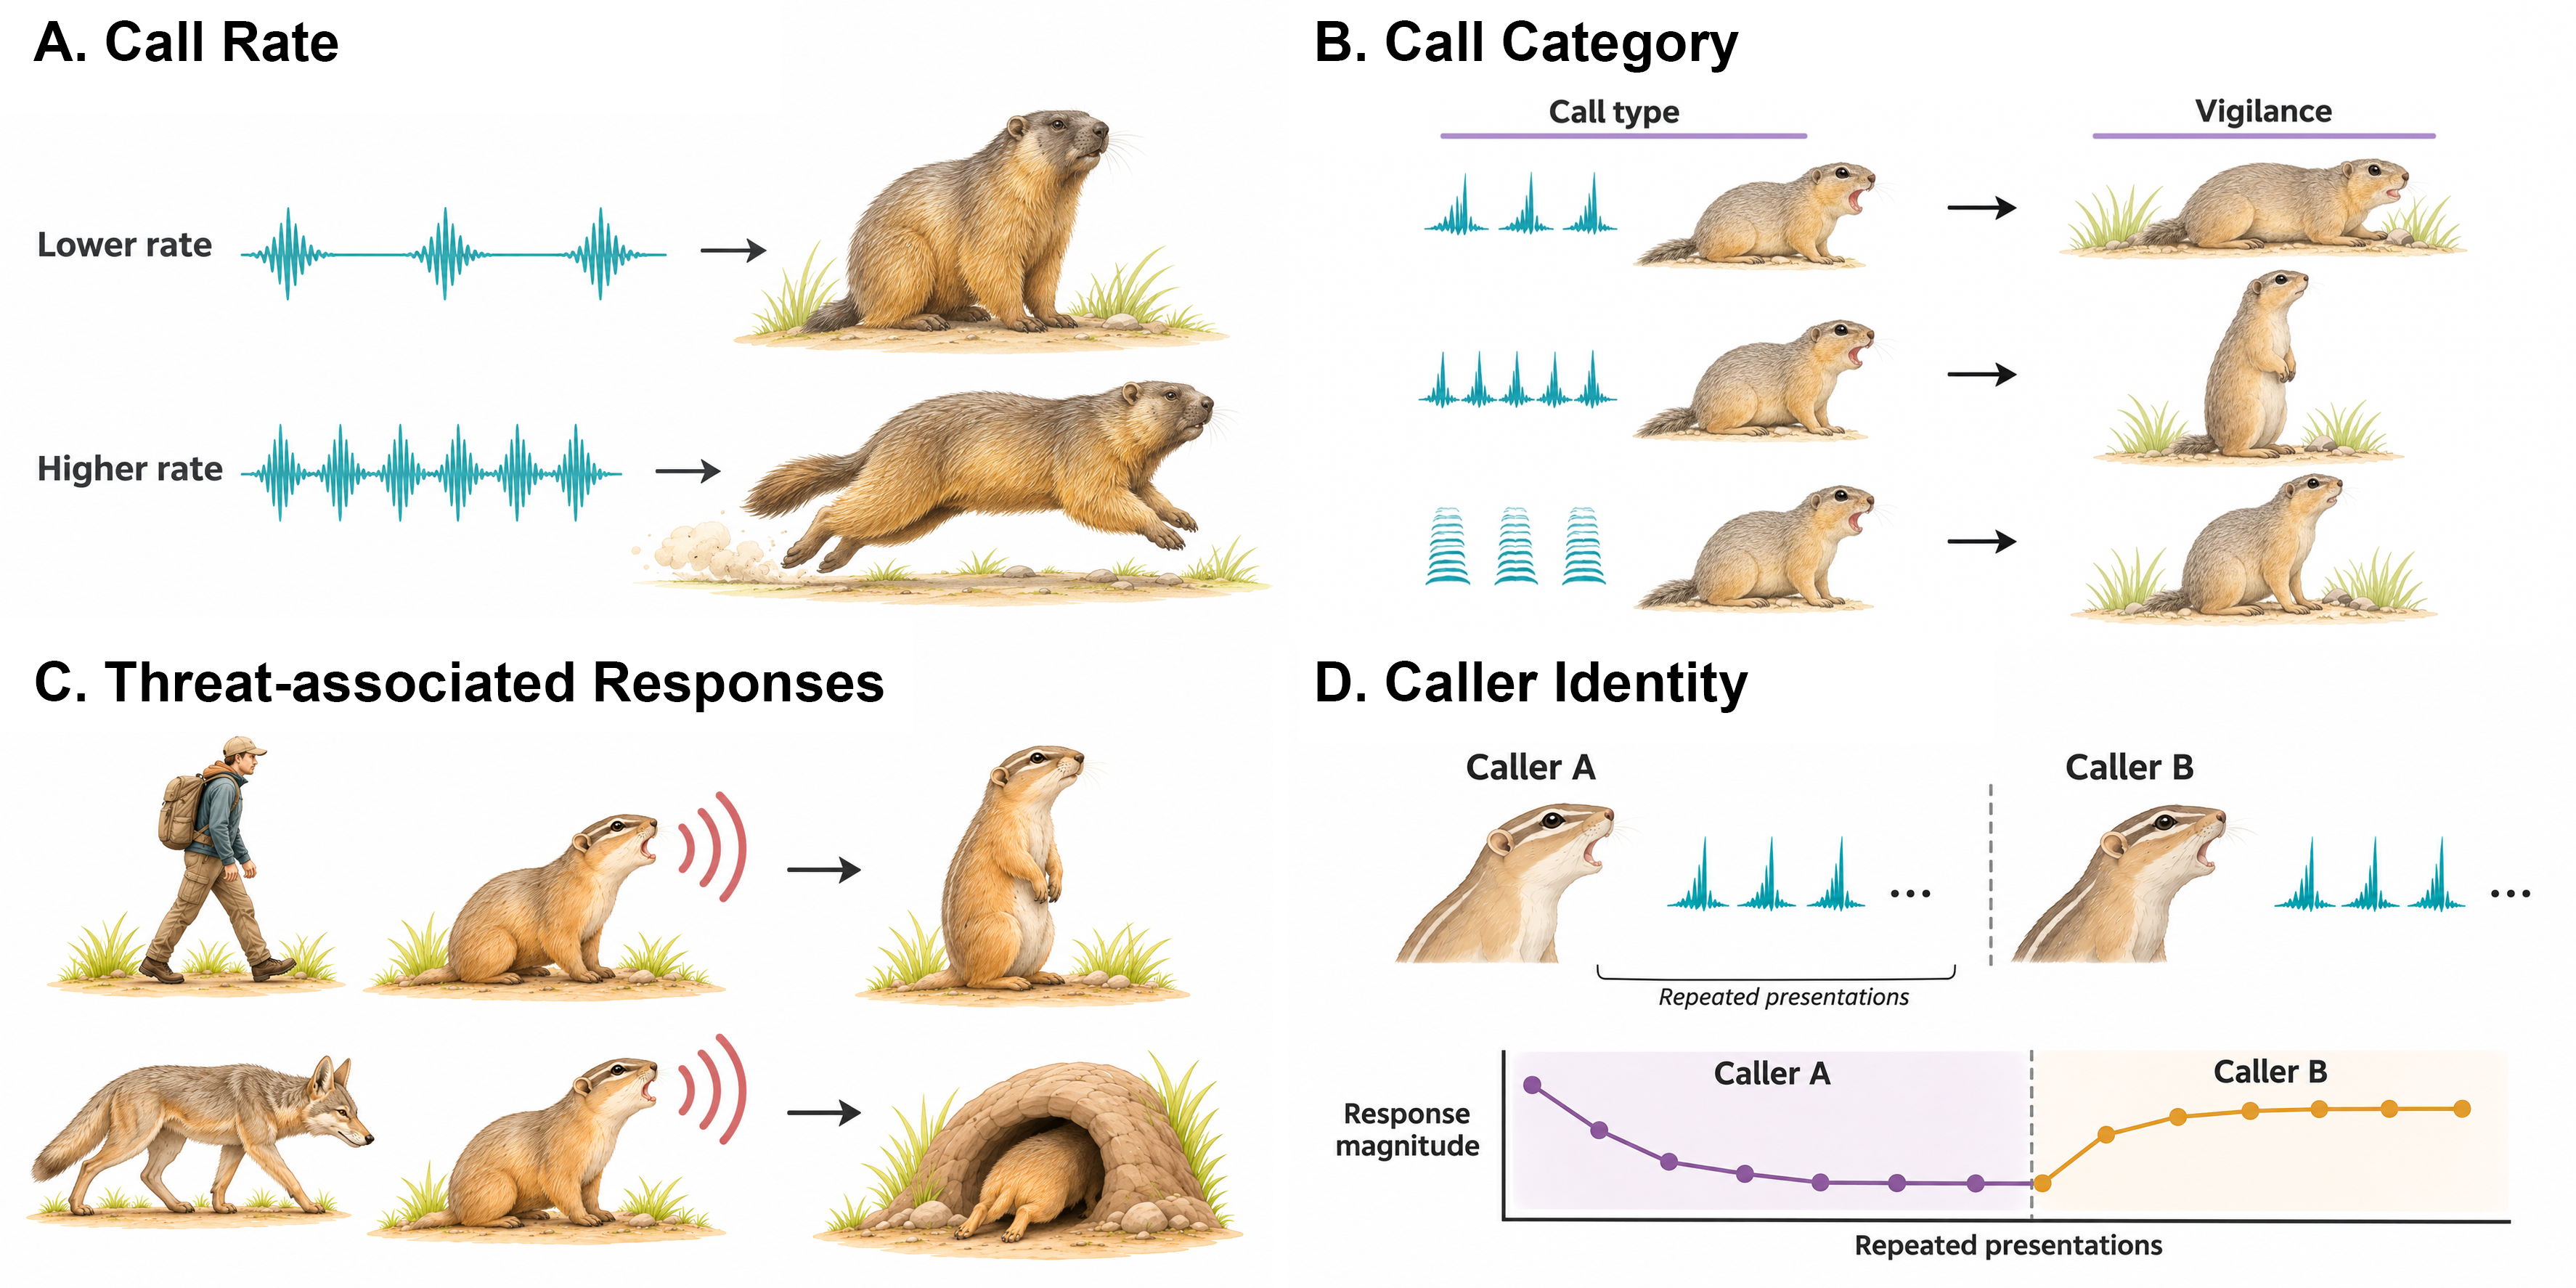
\includegraphics[width=\textwidth]{fig2_designspace.png}
  \caption{Different forms of acoustic information across rodent alarm systems. (A)~Alarm-call rate in yellow-bellied marmots conveys risk-related information, with higher rates associated with stronger antipredator responses \citep{BlumsteinArmitage1997}. (B)~Richardson's ground squirrels distinguish alarm-call categories and exhibit corresponding differences in vigilance \citep{SloanEtAl2005}. (C)~Gunnison's prairie dog alarm calls elicited by different threats, including humans and coyotes, can evoke threat-associated escape responses during playback, indicating that calls convey information beyond generalized urgency \citep{KiriazisSlobodchikoff2006}. (D)~Responses can decline across repeated presentations from one caller and recover when the caller changes, demonstrating source-specific response updating without necessarily establishing reliability learning \citep{Hare1998}. Acoustic representations, behavioral illustrations, and response curves are schematic rather than measured data; specific illustrated postures do not imply experimentally established stimulus--response mappings. Together, these examples illustrate that rodent alarm systems convey different kinds of information rather than a universal predator or urgency code. Schematic illustration created with ChatGPT (OpenAI) image generation and verified by the author.}
  \label{fig:info-kinds}
\end{figure}

Yellow-bellied marmot (\textit{Marmota flaviventer}) alarms do not map onto predator species. Instead, call rate and some acoustic parameters track risk, and receivers use rate as risk information \citep{BlumsteinArmitage1997}.
% VERIFY: BlumsteinRecapet2009, SloanEtAl2005, SwanHare2008 (not full-text checked where marked).
Adding noisy, nonlinear components to marmot calls reduces foraging more than unmanipulated calls do \citep{BlumsteinRecapet2009}. Richardson's ground squirrels adjust vigilance differently to chirps, whistles, and chucks \citep{SloanEtAl2005}, and the first syllables of repeated calls are strongly alerting \citep{SwanHare2008}. Gunnison's prairie dogs (\textit{Cynomys gunnisoni}) are a contrasting case. Playback of alarm calls previously elicited by humans, dogs, or coyotes reproduces the corresponding escape behavior, whereas a control matched in rhythm, frequency range, and amplitude does not \citep{KiriazisSlobodchikoff2006}. The calls carry enough information for predator-specific escape; this does not require that they function as words, and it has not been shown for other sciurids. Urgency coding and predator-associated categories are different informational solutions, and resisting a universal claim about ``what alarm calls mean'' is part of the comparative point.

Who is calling is itself information. Marmots respond more to juvenile than to adult-female calls but do not distinguish familiar from unfamiliar callers \citep{BlumsteinDaniel2004}. Caller identity is carried by rat 50-kHz calls \citep{VielleEtAl2021} and by prairie vole calls \citep{WarrenEtAl2025}.
% VERIFY: WarrenEtAl2025, SchmidtEtAl2008 (not full-text checked).
Nor is relevance ranked by whether the source is a predator. Eastern chipmunks (\textit{Tamias striatus}) change their foraging more to titmouse mobbing calls than to hawk calls \citep{SchmidtEtAl2008}: an indirect social cue can outweigh a predator's own voice.

\subsection{Interpretation depends on experience and social ecology}
\label{sec:features-experience}

A sound can be ecologically relevant without being recognized innately. Tests of predator-call recognition in predator-naïve laboratory rodents disagree. Male DBA/2 mice show defensive responses to owl calls \citep{HendrieNeill1991}, whereas C57BL/6J mice, Sprague-Dawley rats, and gerbils show no selective defense relative to non-predator calls \citep{KindermannEtAl2009}. Species, strain, sound level, and endpoint all differ; a lack of freezing does not mean a lack of acoustic processing; and the variation across paradigms rules out a simple innate-versus-learned answer. Rodents with field experience respond more consistently, though in different ways: voles may freeze or flee, while spiny mice show hormonal change without overt behavior \citep{EilamEtAl1999,HendrieEtAl1998}.

Rat 22-kHz calls show the role of experience most clearly. Selective freezing to these calls depends on prior aversive experience \citep{KimEtAl2010,EndresEtAl2007}, and preventing a rat from calling during its own shock does not abolish later freezing to the calls \citep{CalubEtAl2018}. Yet naïve rats still slow their movement and heart rate to natural 22-kHz calls \citep{OlszynskiEtAl2020}, so ``no response without experience'' is true only if freezing is the sole measure. In the field, eavesdropping on other species' alarms reflects both familiarity and acoustic similarity \citep{GetschowEtAl2013,Shriner1998}, and receivers also use other species' sounds as signals of safety \citep{LillyEtAl2019}.

\subsection{The generality problem}
\label{sec:features-generality}

Which of these findings reflect learned associations specific to a species, which reflect general acoustic biases (rough or abrupt sounds as attention-grabbing, for example), and which depend on social ecology? Telling these apart requires acoustically controlled variants presented to receivers with different associative histories, with the same endpoints measured in laboratory and field animals. Few studies provide both. Unmatched controls, single sound levels, unreported calibration, and strain differences are therefore not technical footnotes; they limit what can be inferred about the information a sound carries.

The same acoustic feature can also feed different downstream systems. Frequency or timing codes that support discrimination need not engage the circuits that select freezing, flight, or autonomic change, and abrupt or looming sounds can trigger defense through fast routes that bypass learned meaning (\secref{sec:mechanisms}). These tensions recur when laboratory and field receivers are compared in \secref{sec:action} and \tabref{tab:comparison}.
